\section{Experiments}

We evaluate \coolname{} on a real-world robot setup to study three questions: whether latent world-model rollouts preserve task-relevant information for value-based ranking, whether \coolname{} improves robustness under deployment-time distribution shift, and how action diversity and value-guided steering contribute to performance. Across all experiments, \coolname{} is \textbf{used zero-shot}, i.e. none of the policy, world model, or value model components are finetuned on data from the target evaluation environment.

\subsection{Real Robot Setup}

Our experiments follow the DROID setup using a 7-DoF Franka Panda manipulator with a Robotiq two-finger gripper. Compared to the original DROID configuration, we replace the exterior cameras with Intel RealSense L515 cameras and mount the robot on a static workbench.
\textbf{All evaluations are conducted in a different lab environment}, introducing a different robot instance, low-level controller, camera configuration, background, lighting, and object distribution relative to \coolname{} development. These changes occur simultaneously, resulting in substantial distribution shift.







\subsection{Evaluating the World Model}

\begin{figure}[t]
\centering

\begin{minipage}[t]{0.38\textwidth}
    \centering
    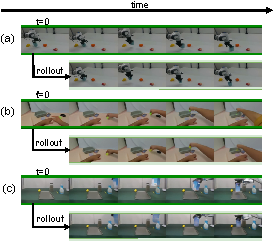
\includegraphics[width=\linewidth]{figures/wm_rollout.pdf}

    \caption{\textbf{World model rollouts across multiple embodiments.}
    Only a single camera view is visualized for clarity.}
    \label{fig:rollout}
\end{minipage}
\hfill
\begin{minipage}[t]{0.58\textwidth}
    \centering

    \vspace{-120pt} % change height

    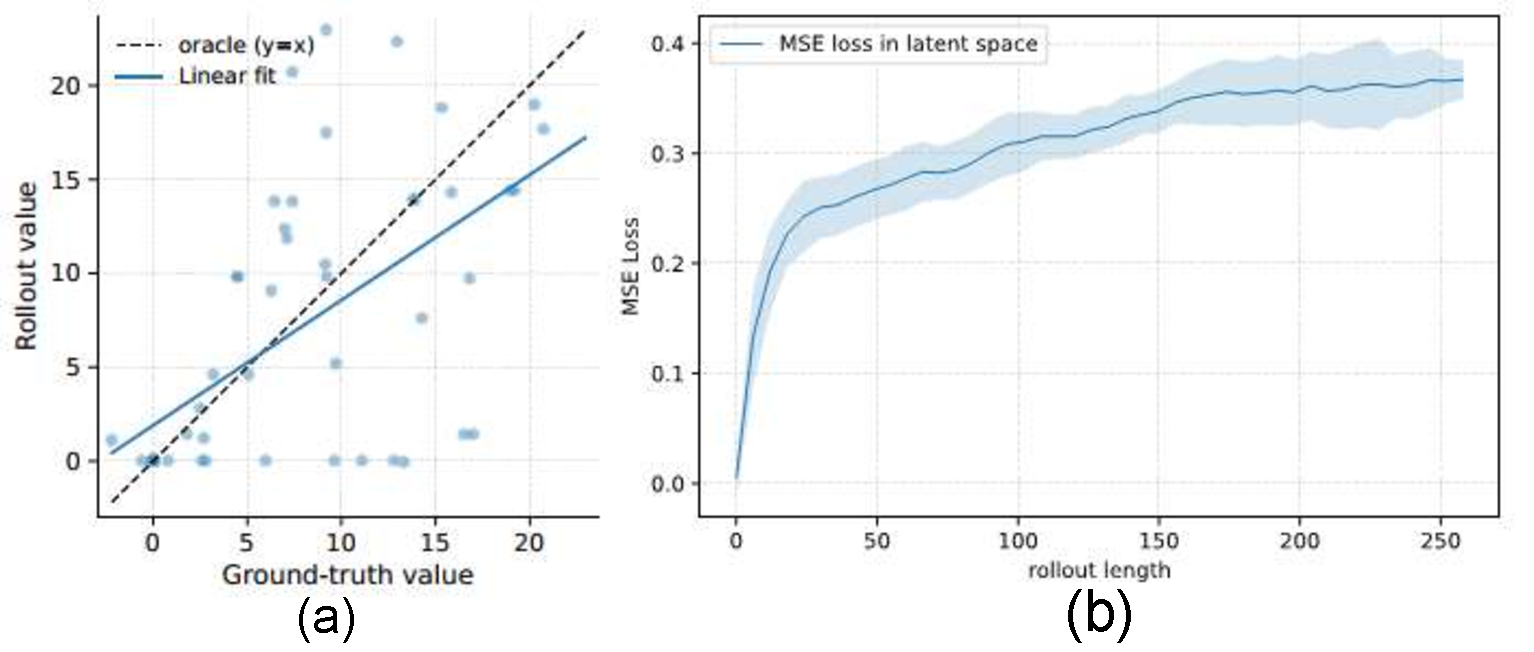
\includegraphics[width=\linewidth]{figures/wm_eval.pdf}

    \caption{\textbf{Evaluative consistency of imagined rollouts.} (a) Value-model scores on ground-truth and imagined trajectories. (b) Latent prediction error versus rollout length; shaded area denotes $\pm$1 standard deviation.}
    \label{fig:VLAC_eval}
\end{minipage}

\end{figure}






% \begin{wrapfigure}{r}{0.5\textwidth}
%     \centering
%     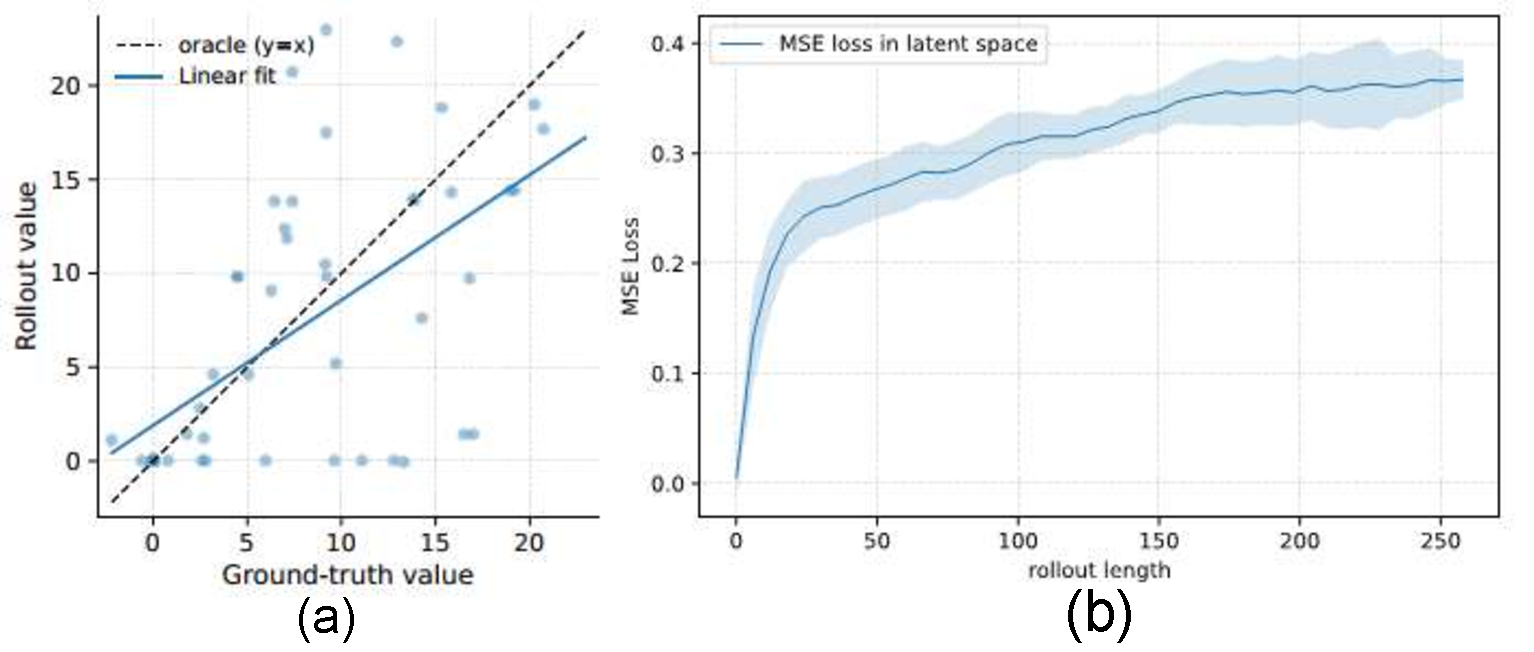
\includegraphics[width=\linewidth]{figures/wm_eval.pdf}
%     \caption{\textbf{Evaluative consistency of imagined rollouts.} (a) Value-model scores on ground-truth and imagined trajectories. (b) Latent prediction error versus rollout length; shaded area denotes $\pm$1 standard deviation.}
%     \label{fig:VLAC_eval}
% \end{wrapfigure}




We first evaluate whether latent world model rollouts preserve the relative value trends needed for trajectory ranking. \coolname{} does not require calibrated reward prediction or photorealistic video generation, only imagined rollouts that preserve relative ranking consistency across candidate action chunks. The rollout results are shown in Fig.~\ref{fig:rollout}. 
% More visualizations will be shown in supplementary material.
We compare value-model scores on short ground-truth video clips and corresponding imagined rollouts generated from action chunks with horizon $H{=}10$ under the same language instructions. As shown in Fig.~\ref{fig:VLAC_eval}(a), the two sets of scores are positively correlated, with Pearson $r=0.66$ (95\% CI $[0.46,0.79]$, $p<10^{-6}$) and Spearman $\rho=0.69$ ($p<10^{-7}$). This consistency is sufficient for rollout ranking in \coolname{}. We also measure latent prediction error as rollout length increases. As shown in Fig.~\ref{fig:VLAC_eval}(b), latent MSE increases gradually over the evaluated horizon, suggesting that the model remains sufficiently stable for repeated short-horizon rollout evaluation. All the data for quantitative evaluation are sampled from the unseen RoboArena dataset~\citep{atreya2025roboarena}.




\subsection{Evaluating \coolname{}}
\label{sec:Eval_dreamsteer}

We evaluate \coolname{} as a complete system with two primary goals: \textbf{(1) improving robustness to out-of-distribution (OOD) objects}, and \textbf{(2) improving instruction-following (IF) accuracy under language-specified constraints}. The OOD objects and the scenes used to evaluate IF accuracy are shown in Fig.~\ref{fig:objects}.

Across all experiments, we use a $\pi_0$ checkpoint pretrained on DROID as the base policy. Unless otherwise specified, we use $K{=}5$ sampled action chunks and horizon $H{=}10$. We use chunk-level steering because imagined observations for $H{=}1$ are often too similar for reliable ranking, while longer action chunks produce more distinguishable future states. Steering is applied once every five control steps for efficiency. Each task is evaluated over 20 trials with randomized object poses and positions. The steering step requires approximately 13\,s of computation. This cost scales with the number of candidate action chunks: generating, rolling out, and evaluating a single candidate requires approximately 1\,s in our implementation, and we use 13 candidates during deployment. Rollout and evaluation are fully parallelizable and could substantially reduce steering latency, as our current implementation prioritizes feasibility over inference optimization.

\begin{figure}[t]
  \centering
  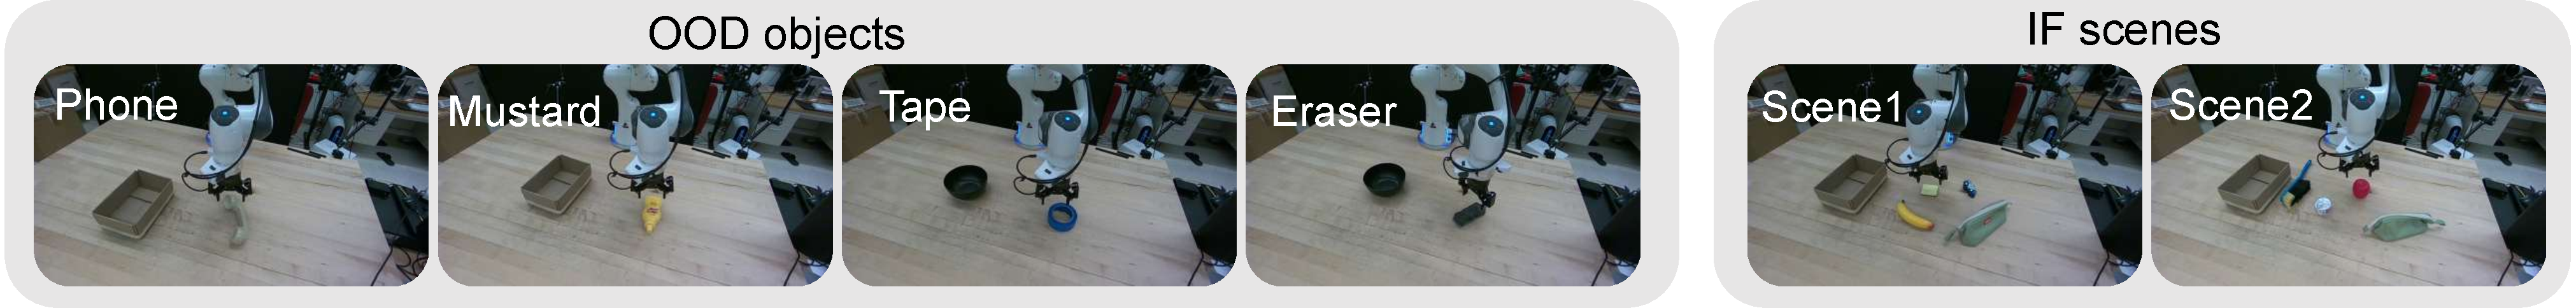
\includegraphics[width=\linewidth]{figures/objects-edit.pdf}
  \caption{\textbf{Real-world evaluation tasks.} Left: OOD object manipulation tasks involving previously unseen objects. Right: instruction-following (IF) scenes containing multiple objects and distractors.}
  \label{fig:objects}
\end{figure}

\paragraph{OOD Object Generalization.}

We evaluate \coolname{} on OOD object manipulation using a standard pick-and-place task, where the robot must place a specified object into a designated receptacle. The task structure is fixed, but the target objects differ from the policy training distribution in appearance, geometry, and material properties, making them challenging for the pretrained policy.
We compare \coolname{} against several ablations: $\pi_0$ denotes single-sample policy execution; $\pi_0$ + \coolname{} ranks multiple $\pi_0$ action chunks; primitives + \coolname{} ranks only predefined Cartesian primitives; and $\pi_0$ + primitives + random selects uniformly at random from the same candidate set as the full method.

As shown in Table~\ref{tab:ood-performance}, \coolname{} improves OOD manipulation success rate from 23.75\% to 66.25\%. Ranking multiple $\pi_0$ samples improves over single-sample execution, suggesting that useful action chunks exist in the policy distribution but are not reliably selected. Primitives alone achieve zero success, while random selection over the same candidate set also fails, indicating that both candidate diversity and value-guided ranking are necessary. The full method performs best by combining diverse policy proposals, primitive-based local exploration, and rollout evaluation.

We also study the effect of proposal count $K$ on the whiteboard eraser task. Increasing $\pi_0$ samples from $K{=}3$ to $K{=}5$ improves success, while increasing further to $K{=}7$ provides little additional benefit but increases rollout cost. We therefore use $K{=}5$ in all experiments.


\begin{table}[h]
\caption{\textbf{OOD object performance.}
Success rates over 20 trials per object. The last column reports the aggregate success rate over all 80 trials with 95\% Wilson confidence intervals.}
\label{tab:ood-performance}

% \vspace{-4pt}
\centering
\scriptsize
\setlength{\tabcolsep}{3.0pt}
\renewcommand{\arraystretch}{0.82}

\begin{tabular}{lcccccc}
\toprule
Method & Phone & Mustard & Tape & Eraser & Average & 95\% CI \\
\midrule
$\pi_0$
& 4/20 & 3/20 & 6/20 & 6/20 & 23.75 & [15.84, 34.07] \\

$\pi_0$ + \coolname{}
& 7/20 & 6/20 & 11/20 & 10/20 & 42.50 & [32.26, 53.43] \\

$\pi_0$ + primitives + random
& 0/20 & 0/20 & 0/20 & 0/20 & 0.00 & [0.00, 4.58] \\

primitives + \coolname{}
& 0/20 & 0/20 & 0/20 & 0/20 & 0.00 & [0.00, 4.58] \\

\midrule
$\pi_0$ + primitives + \coolname{}
& \textbf{12/20}
& \textbf{11/20}
& \textbf{16/20}
& \textbf{14/20}
& \textbf{66.25}
& \textbf{[55.39, 75.65]} \\
\bottomrule
\end{tabular}

\vspace{-6pt}
\end{table}




\paragraph{Instruction Following Accuracy.}

We next evaluate whether \coolname{} improves instruction following in complex scenes.  We report instruction-following accuracy. A trial is counted as correct if the robot makes consistent contact with, or attempts to grasp, the language-specified object. This metric isolates semantic target selection from low-level execution difficulty, allowing us to evaluate whether test-time steering improves adherence to language constraints. As shown in Table~\ref{tab:instruction-following}, \coolname{} improves instruction-following accuracy from 38.75\% to 56.25\%, a gain of 17.5 percentage points over $\pi_0$. These results suggest that imagined rollout scoring helps reject action proposals whose predicted outcomes do not align with the semantic intent of the instruction.




\begin{table}[h]
\caption{\textbf{Instruction following performance.}
Accuracy over 20 trials per target object. The last column reports the aggregate accuracy over all 80 trials with 95\% Wilson confidence intervals.}
\label{tab:instruction-following}

\centering
\scriptsize
\setlength{\tabcolsep}{3pt}
\renewcommand{\arraystretch}{0.82}

\begin{tabular}{lcccccc}
\toprule
Method & Sponge & Banana & Pencil & Apple & Average & 95\% CI \\
\midrule

$\pi_0$
& 8/20 & 9/20 & 6/20 & 8/20
& 38.75
& [28.78, 49.73] \\

\midrule

$\pi_0$ + primitives + \coolname{}
& \textbf{14/20}
& \textbf{13/20}
& \textbf{9/20}
& \textbf{9/20}
& \textbf{56.25}
& \textbf{[45.34, 66.57]} \\

\bottomrule
\end{tabular}

\vspace{-6pt}
\end{table}



% \subsubsection{Behavior Stability and Execution Efficiency}

% Beyond task success and instruction following, we observe that \coolname{} improves the stability of executed behaviors. The base $\pi_0$ policy often produces erratic or oscillatory motions under distribution shift, leading to repeated corrective movements or unstable approach trajectories. By evaluating candidate chunks through imagined rollouts, \coolname{} suppresses some of these undesirable actions and selects smoother, more consistent behavior.

% In our trials, \coolname{} also tends to require roughly half the number of control steps compared to $\pi_0$ on successful OOD executions. This is because suboptimal single-sample actions often require multiple corrective steps to recover, or can lead to failure states from which the policy does not recover. \coolname{} instead evaluates several possible futures before acting, which reduces the number of failure-inducing actions executed on the robot.

% This additional reasoning introduces moderate latency. In our current implementation, policy inference takes 0.08s, world-model rollout takes 0.59s, and value-model evaluation takes 0.37s for an action chunk of horizon $H{=}10$, averaged over 10 runs. In practice, we apply steering once every five control steps, which amortizes planning cost over execution. The current implementation is not optimized for latency; parallel world-model rollouts, KV caching, and more efficient attention implementations such as FlashAttention provide straightforward opportunities for further speedup. We also find that latent rollout is substantially faster than pixel-space video generation~\cite{guo2025ctrl}: on the same NVIDIA RTX 4090 setup, generating three $320{\times}192$ frames at horizon $H{=}10$ takes 23.12s with a video diffusion model, compared to 0.59s for our latent world model.





% \subsection{Failure Analysis}
% \label{sec:failure_analysis}

% Despite the overall performance gains reported in Section~\ref{sec:Eval_\coolname{}}, \coolname{} still exhibits failure modes that reflect limitations of its predictive and evaluative components. These failures are useful to analyze because \coolname{} explicitly exposes where errors arise: candidate generation, imagined rollout, or value-based ranking.

% \paragraph{World Model Hallucination}
% While rare in our experiments, the action-conditioned world model occasionally predicts a successful grasp in imagination even when the real robot fails to establish a grasp. We refer to this as a ``magic grasp'' hallucination: the decoded rollout shows the object being grasped or lifted, while the real execution leaves the object behind. We attribute this behavior to bias in the world-model training data toward successful manipulation trajectories, which can cause the model to overestimate grasp feasibility under uncertainty. When candidate actions induce such over-optimistic rollouts, the value model may fail to reject physically infeasible actions. A practical mitigation is to expand world-model training beyond success-biased demonstrations by incorporating failure trajectories and random-play interaction data. These data expose the model to missed grasps, slips, non-graspable contacts, and unsuccessful attempts, reducing the bias that leads to unrealistic rollouts. Qualitative examples of these failure cases are provided in the supplementary material.

% \paragraph{Value Model Misranking}
% A second failure mode arises from imperfect ranking by the value model. While generally effective, the value model is sensitive to viewpoint and visual presentation. In our current system, scoring is performed from a single fixed camera view, which can make some action outcomes visually ambiguous or partially occluded. As a result, the highest-scoring imagined trajectory does not always correspond to the best real-world action. A natural improvement is to provide the value model with multiple camera views and aggregate scores across views, for example by averaging. This would reduce sensitivity to viewpoint-specific ambiguities and make the ranking more robust under occlusion.



